\section{A simple example: classify handwritten digits with a multi-layer
  perceptron}

\begin{frame}
  \frametitle{The MNIST dataset}
  \begin{columns}
    \begin{column}{0.5\textwidth}
      \begin{itemize}
      \item Classic dataset
        \begin{itemize}
        \item Lots of methods have been tested with it
        \end{itemize}
      \item The task is to recognize the digit on the image
      \item All images have the same size and aspect ratio (non-trivial
        pre-processing)
      \item The label is known
      \end{itemize}
    \end{column}
    \begin{column}{0.5\textwidth}
      \begin{tikzpicture}[>=stealth]
        \node[anchor=south west,inner sep=0] (image) at (0,0) {
          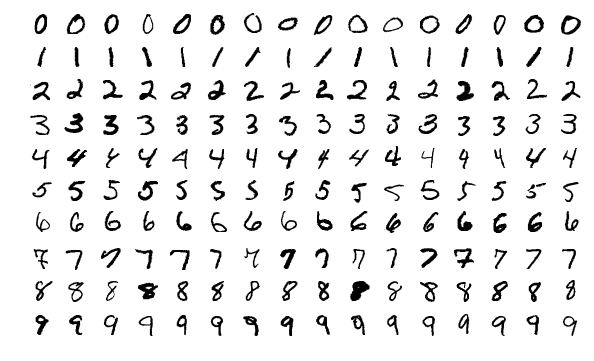
\includegraphics[width=\columnwidth]{img/MnistExamples.png}
        };
        \onslide<2->{
        \begin{scope}[x={(image.south east)},y={(image.north west)}]
          \draw[red,ultra thick] (0.22,0.15) rectangle (0.28,0.25);
        \end{scope}
        }
      \end{tikzpicture}
      \url{http://yann.lecun.com/exdb/mnist/index.html}
    \end{column}
  \end{columns}
\end{frame}

\begin{frame}
  \frametitle{Multi-layer perceptron: computation}
  \begin{textblock}{50}(0,10)
    \begin{itemize}
    \item 1957 but many improvements since
    \item<2-> Input layer
      \begin{itemize}
      \item flatten image: $\output^{1}_{k} = \matrixLinElem{\matrix{I}}{k}$
      \end{itemize}
    \item<3-> Hidden layers
      \begin{itemize}
      \item Weighted sum:
      \item Activation function:\\
        ReLU $\output^{\layer+1}_{k}$
      \end{itemize}
    \item<4-> Output layer
      \begin{itemize}
      \item Softmax:
      \end{itemize}
    \end{itemize}
  \end{textblock}
  \begin{textblock}{70}(30,20)
    \begin{tikzpicture}[>=stealth]
      % Inspired by https://tex.stackexchange.com/a/153974

      % Input image and grid
      % This part is inspired by https://tex.stackexchange.com/a/128648
      % and a lot of trial and error for the grid (including a bit of ChatGPT)
      % Apparently, the idea is to fix the size of the image and then the grid
      % flows
      % I use 56px (twice the real size) so that it looks OK and computations are easy.
      \def\xInputImage{0}
      \def\nameInputImage{input-name}
      \node[anchor=center,inner sep=0pt,draw=black] (\nameInputImage) at (\xInputImage,0) {
        
\includegraphics[width=56px,height=56px]{img/Mnist_8.png}
      };
      \begin{scope}
        \clip (\nameInputImage.south west) rectangle (\nameInputImage.north east);
        \draw[step=2px,gray,very thin] (\nameInputImage.south west) grid (56px, 56px);
      \end{scope}

      \onslide<2->{
      % Input layer
      \def\xInput{1.8}
      \def\nameInput{input}
      \node [align=center, above] at (\xInput,2.2) {Input \\ layer \\ {\tiny $28\times28=784$ units}};
      \foreach \m/\l [count=\y] in {1,2,3,missing,4}
      \node [every neuron/.try, neuron \m/.try] (\nameInput-\m) at (\xInput,3.0-\y) {};

      % Connections from input image to input layer
      % No loop here cause we need to shift the positions
      % It uses the scale introduced above
      \draw [->] (\nameInputImage)++(-27px,27px) -- (\nameInput-1);
      \draw [->] (\nameInputImage)++(-25px,27px) -- (\nameInput-2);
      \draw [->] (\nameInputImage)++(-23px,27px) -- (\nameInput-3);
      \draw [->] (\nameInputImage)++(27px,-27px) -- (\nameInput-4);
      }

      \onslide<3->{
      % First hidden layer
      \def\xHiddenI{3.6}
      \def\nameHiddenI{hidden1}
      \node [align=center, above] at (\xHiddenI,2.2) {Hidden \\ layer \\ {\tiny 200 units}};
      \foreach \m [count=\y] in {1,2,missing,3}
      \node [every neuron/.try, neuron \m/.try ] (\nameHiddenI-\m) at (\xHiddenI,2.5-\y) {};

      % Connections from input layer to first hidden layer
      \foreach \i in {1,...,4}
      \foreach \j in {1,...,3}
      \draw [->] (\nameInput-\i) -- (\nameHiddenI-\j);

      % Second hidden layer
      \def\xHiddenII{5.4}
      \def\nameHiddenII{hidden2}
      \node [align=center, above] at (\xHiddenII,2.2) {Hidden \\ layer \\ {\tiny 150 units}};
      \foreach \m [count=\y] in {1,2,missing,3}
      \node [every neuron/.try, neuron \m/.try ] (\nameHiddenII-\m) at (\xHiddenII,2.2-0.9*\y) {};

      % Connections to first hidden layer to second hidden layer
      \foreach \i in {1,2,3}
      \foreach \j in {1,2,3}
      \draw [->] (\nameHiddenI-\i) -- (\nameHiddenII-\j);
      }

      % Output layer
      \def\xOutput{7.2}
      \def\nameOutput{output}
      \node [align=center, above] at (\xOutput,2.2) {Output \\ layer \\ {\tiny 10 units}};
      \foreach \m [count=\y] in {0,1,missing,9}
      \node [every neuron/.try, neuron \m/.try ] (\nameOutput-\m) at (\xOutput,1.8-0.7*\y) {};

      \onslide<4->{
      % Connection from second hidden layer to output layer
      \foreach \i in {1,2,3}
      \foreach \j in {0,1,9}
      \draw [->] (\nameHiddenII-\i) -- (\nameOutput-\j);
      }

      % Output probabilities
      \def\xProba{7.7}
      \def\nameProba{proba}
      \def\missing{missing}
      \foreach \m [count=\y] in {0,1,missing,9}
      \node (\nameProba-\m) at (\xProba,1.8-0.7*\y) {\ifx\m\missing\else {\tiny $\prob{\m}$}\fi};

    \end{tikzpicture}

  \end{textblock}
\end{frame}
